\subsection{Red Laboratorios DC}

Para este experimento, capturamos los paquetes de la LAN Wi-Fi Laboratorios-DC del Departamento de Computació de la FCEyN de la UBA. La medición fue realizada un día Lunes desde las 15hs y durante 15 minutos. La cantidad de paquetes capturados es de 4000. De todos estos, sólo 164 corresponden al protocolo ARP.

\begin{figure}[H]
       \centering
       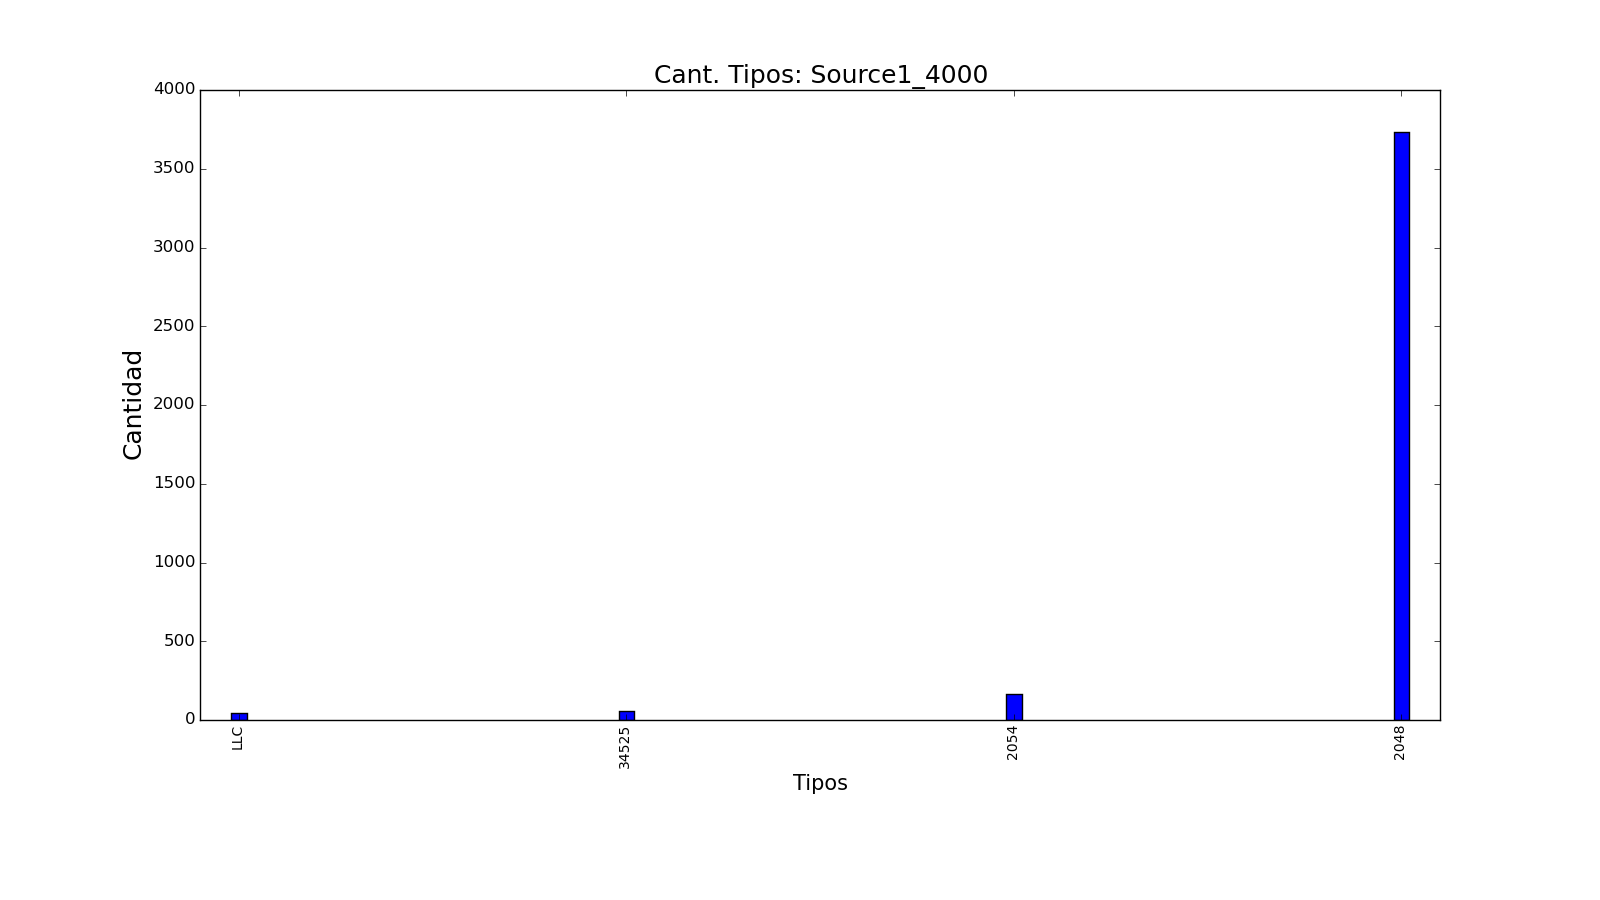
\includegraphics[width=1\textwidth]{../resultados/labo-corrida3/histogram_types.png}
       \caption{Protocolos de los paquetes capturados}
       \label{red-hogarena-types}
\end{figure}

\begin{figure}[H]
       \centering
       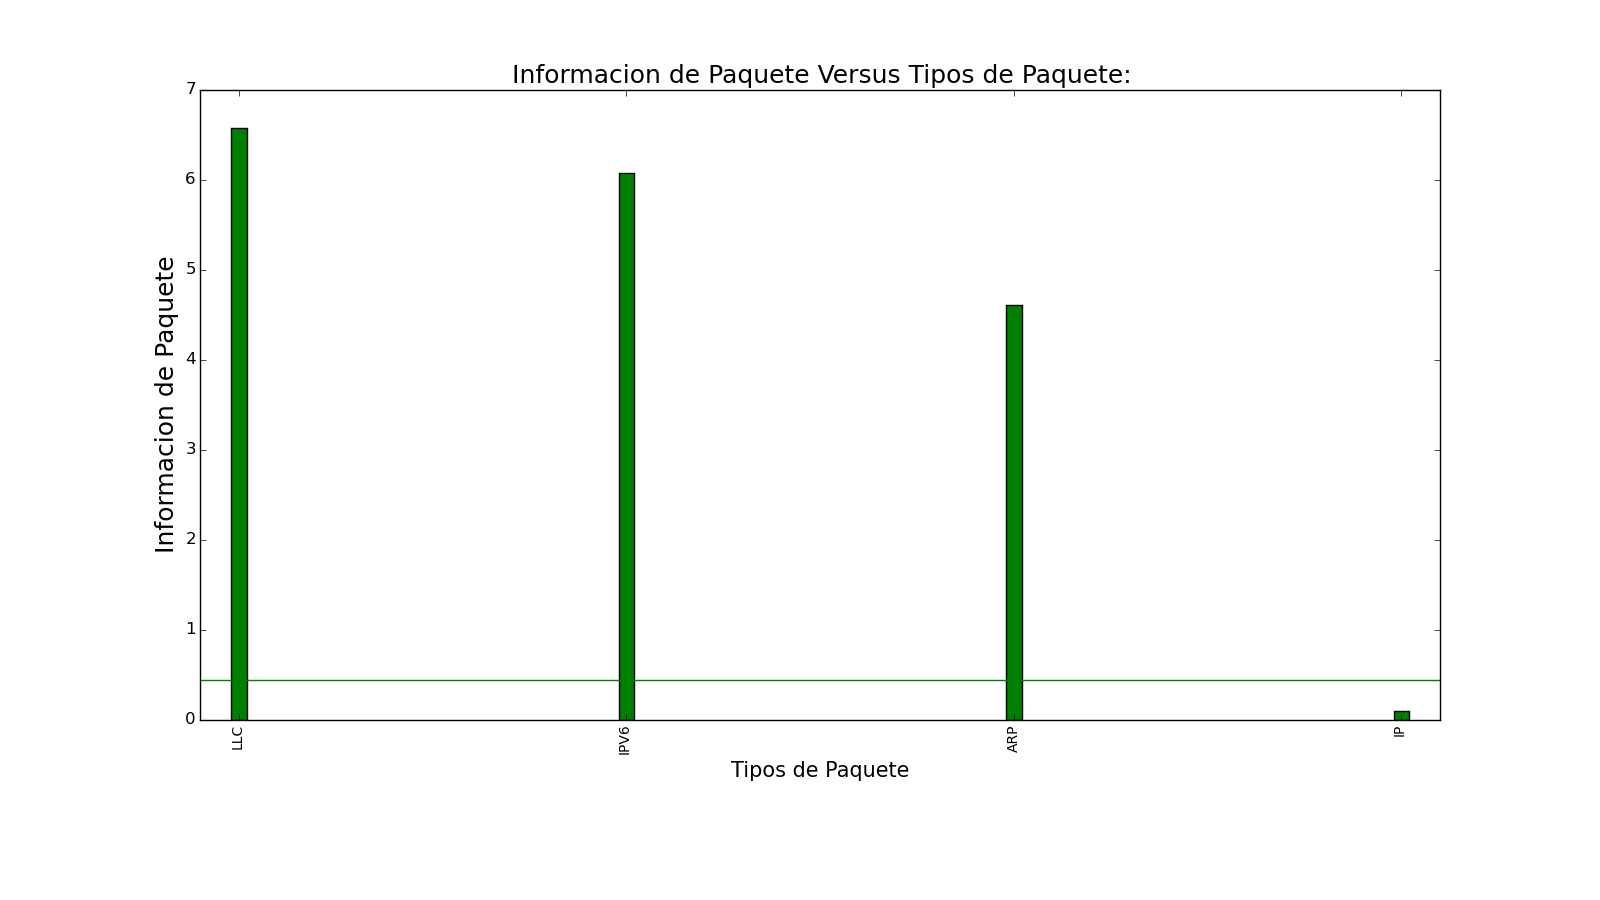
\includegraphics[width=1\textwidth]{../resultados/labo-corrida3/histogram_types_information.png}
       \caption{Información de los protocolos de los paquetes capturados}
       \label{red-hogarena-types-info}
\end{figure}


\begin{figure}[H]
       \centering
       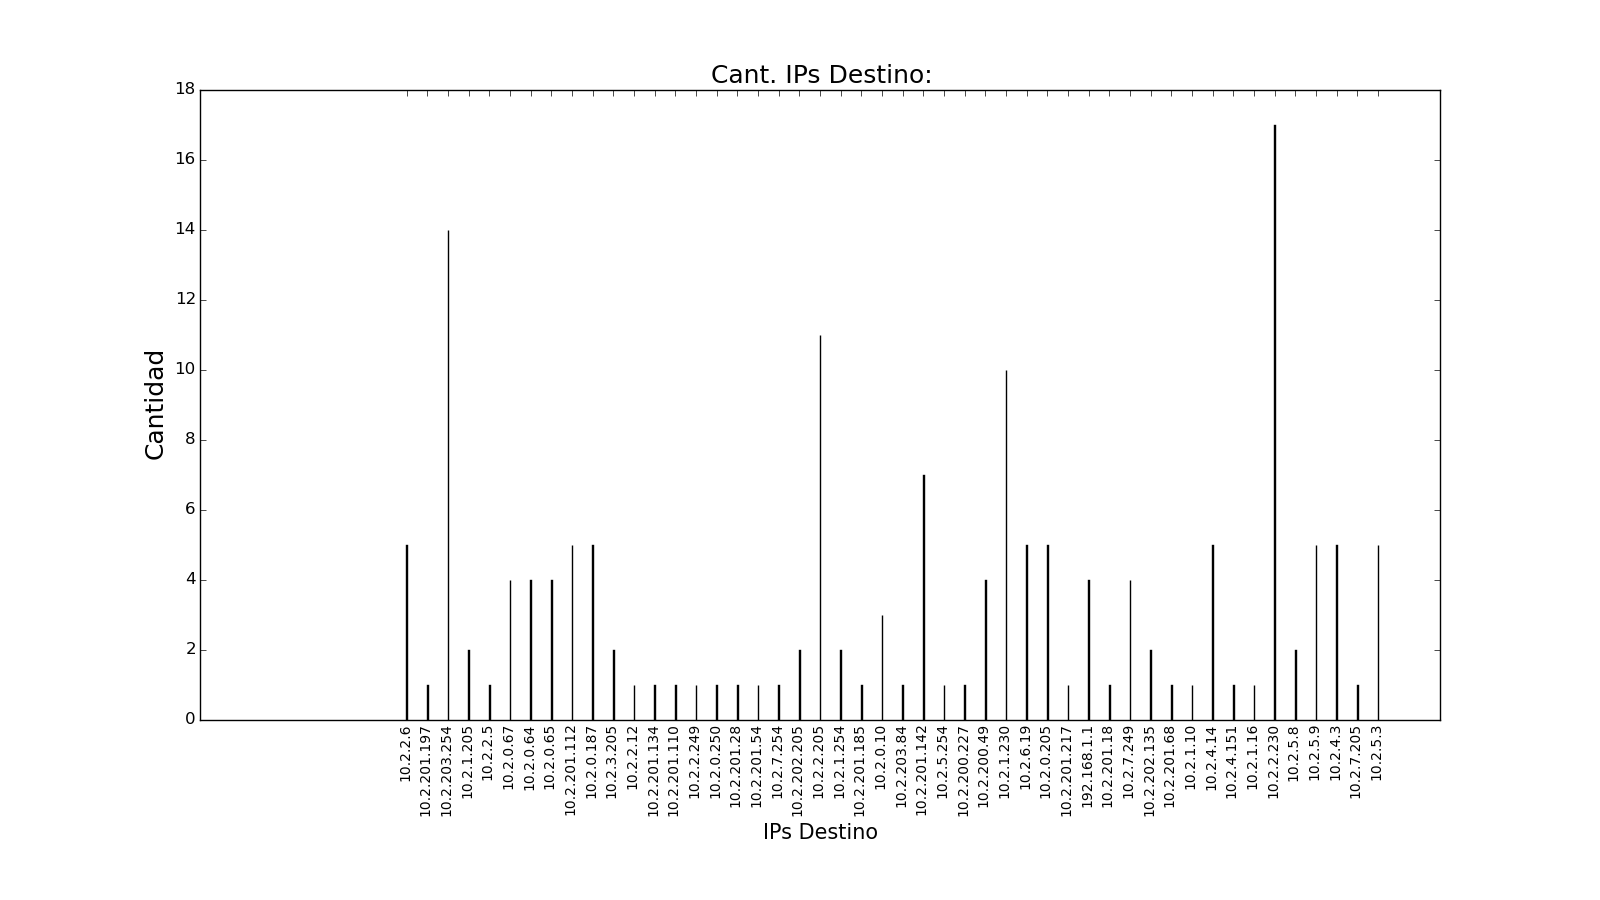
\includegraphics[width=1\textwidth]{../resultados/labo-corrida3/histogram_dst.png}
       \caption{IPs destino de los paquetes ARP}
       \label{red-hogarena-arp-destination}
\end{figure}

\begin{figure}[H]
       \centering
       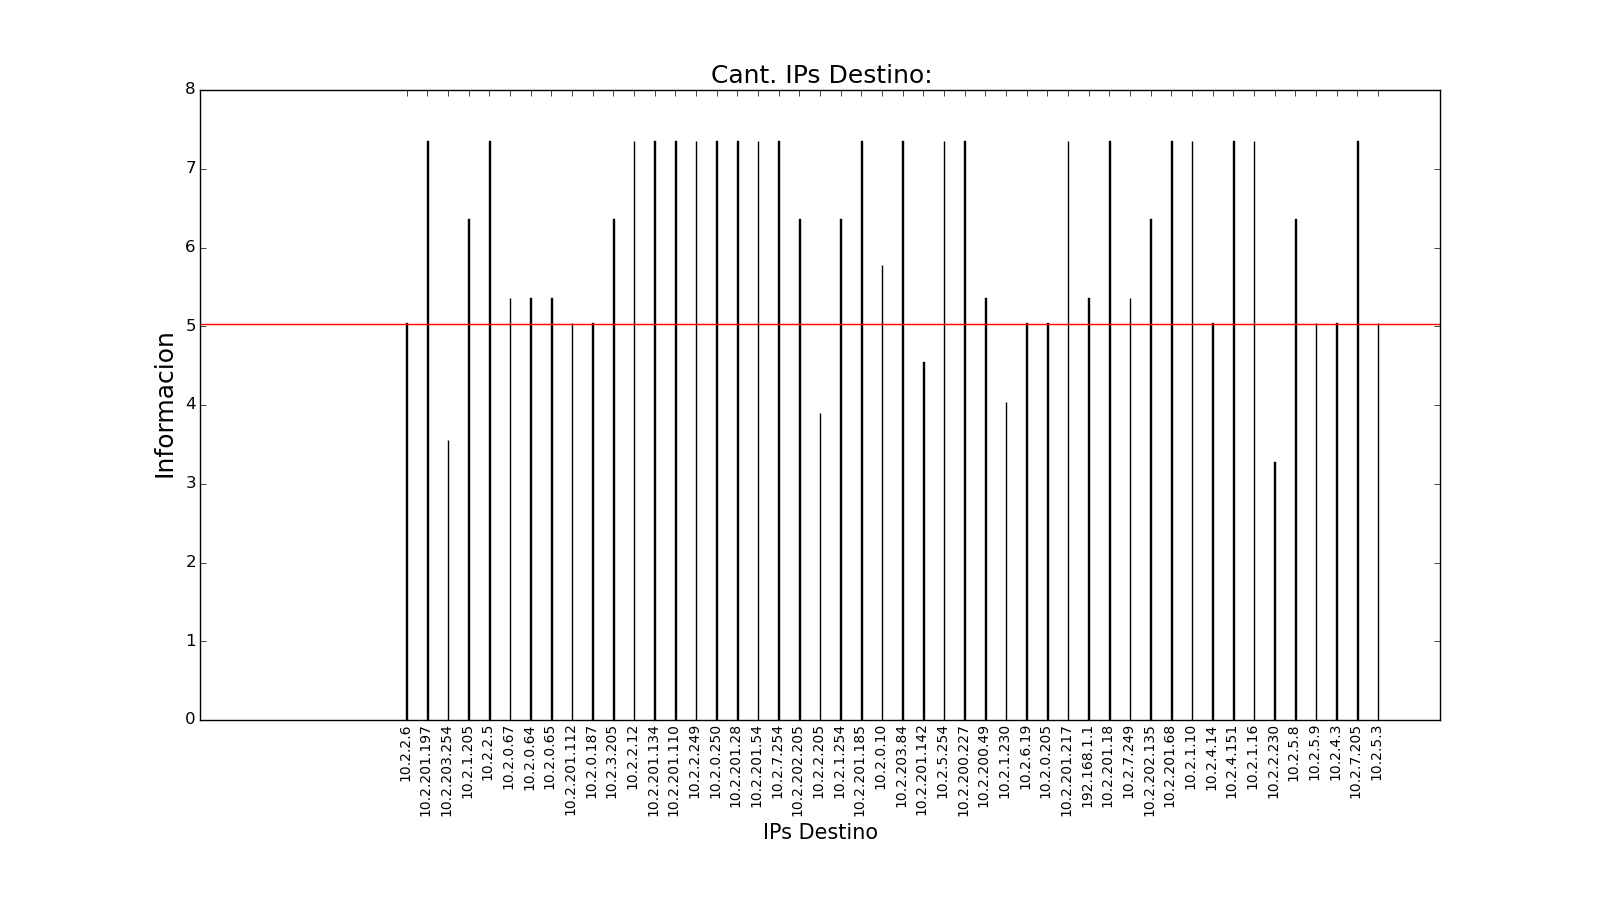
\includegraphics[width=1\textwidth]{../resultados/labo-corrida3/histogram_dst_information.png}
       \caption{Información de IPs destino de los paquetes ARP}
       \label{red-hogarena-arp-destination-info}
\end{figure}

\begin{figure}[H]
       \centering
       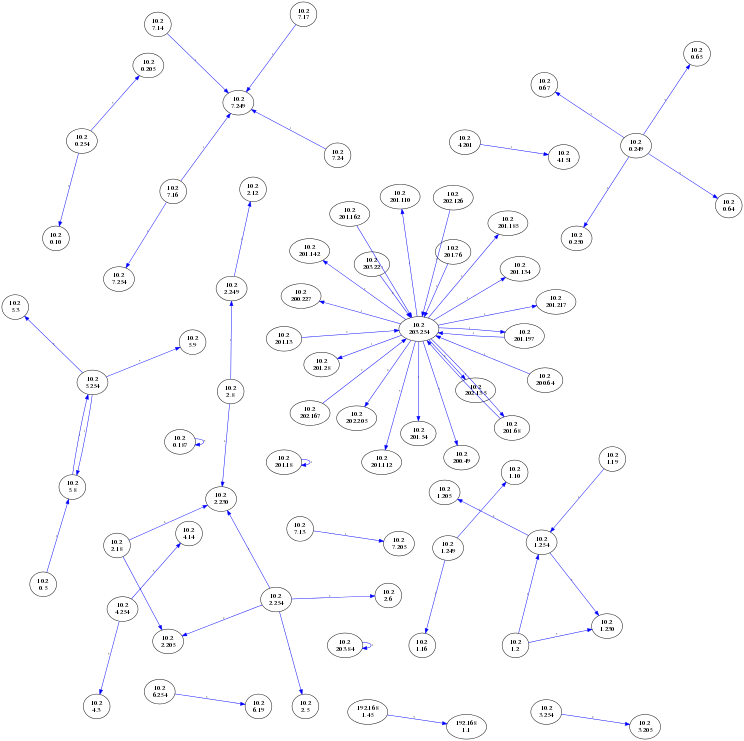
\includegraphics[width=1\textwidth]{../resultados/labo-corrida3/network.png}
       \caption{Tráfico de paquetes ARP}
       \label{red-hogarena-arp-traffic}
\end{figure}

